\documentclass[12pt]{article}
\usepackage[utf8]{inputenc}
\usepackage{float}
\usepackage{amsmath}
% add packages you want to use
% you will submit generated .pdf file on odtuclass
% not the .tex file
% mind that your .pdf file can contain only
% searchable images


\usepackage[hmargin=3cm,vmargin=6.0cm]{geometry}
%\topmargin=0cm
\topmargin=-2cm
\addtolength{\textheight}{6.5cm}
\addtolength{\textwidth}{2.0cm}
%\setlength{\leftmargin}{-5cm}
\setlength{\oddsidemargin}{0.0cm}
\setlength{\evensidemargin}{0.0cm}

\usepackage{tikz}
\usetikzlibrary{automata,positioning}

\begin{document}

\section*{Student Information} 
% Write your full name and id number between the colon and newline
% Put one empty space character after colon and before newline
Full Name : Zeynep Özalp \\
Id Number : 2237691 \\

% Write your answers below the section tags
\section*{Answer 1}
Let $\Sigma=\{0,1\}$. $A_k$ is clearly finite since $A_k$ has a partitioning $S_1,S_2...S_k$ where each $S_i$ is the set of strings of length $i$. The cardinality of $S_i$ is $i^2$. All $S_i$'s are finite. Union of these finite sets are also finite. $B$ is a language and it is countably infinite. The set of strings $\Sigma^*$ is countably infinite and $2^{\Sigma^*}$ is uncountable by theorem 1.5.2 on page 28. So, C is uncountable. 
\subsection*{a.}
The difference of an uncountable set and a finite set is uncountable.
\subsection*{b.}
$$L^*=\Sigma^*$$
1) $L\subseteq\Sigma^* \rightarrow L^*\subseteq \Sigma^{**}=\Sigma^*$. Therefore, $ L^*\subseteq \Sigma^*$.\\
2) $(\{0,1\}\subseteq L) \rightarrow (\{0,1\}^* \subseteq L^*) \rightarrow (\Sigma^* \subseteq L^*)$\\

So, $B^*=\{0,1\}^*$. Thus, the intersection of $2^{\Sigma^*}, \Sigma^*$ and $A_7$ is $A_7$ and it is finite. $|A_7|=49$
\subsection*{c.}
Countably infinite since $\bigcup C =\{0,1\}^*$, $A_2 \times K$ is the set of tuples and $\bigcup C \cap (A_2 \times K) = \{\} $. So, $\bigcup C - (A_2 \times K) = \bigcup C$.
\subsection*{d.}
Countable and its cardinality is 0 since $\bigcup C =\bigcup _{k=1}^\infty A_k=\{0,1\}^*$.

\section*{Answer 2}

\subsection*{a.}
For $s$, there can be 4 different initial states. For $F$, there can be as many as the power set of $K$, which is $2^4$. For $\delta$, the transition function is from $K \times \Sigma$ to $K$. There are $2^3$ tuples in $K \times \Sigma$. These tuples can map to only one state.  So, there are $4^8=2^{16}$ different delta functions. Therefore, $2^2*2^4*2^5=2^{22}$ different DFA can be constructed.
\subsection*{b.}
For $s$, there can be 4 different initial states. For $F$, there can be as many as the power set of $K$, which is $2^4$. For $\Delta$, the transition function is $\Delta \subseteq K \times (\Sigma \cup \{e\})\times K$. There are $4.3.4=48$ different tuples and the transition function can be any subset of these tuples. So, there are $2^{48}$ different transition functions. Therefore, $2^2*2^4*2^{48}=2^{54}$ different NFA can be constructed.
\subsection*{c.}
In NFA's, one configuration can yield to many different configurations but in DFA's, one configuration can yield to only another configuration. Also, in NFA's, machine can pass to another state without reading an input symbol. Because of these reasons, the number of transition functions and the number of M's are clearly different. 
\subsection*{d.}
The number of different FA's are equal to the number of different languages.

\section*{Answer 3}


\subsection*{a.}
$$0^*(100^*100^*100^*100^*)^*0^*\cup 0^*(0^*010^*010^*010^*01)^*0^*$$
\subsection*{b.}
$$(0\cup 1)(01\cup 00)^*\cup (10\cup 00)^*(0\cup 1)$$
\subsection*{c.}
$$1^*((00)(01\cup 10\cup 1)^*(00))^*1^*(e\cup 0)1^*$$



\section*{Answer 4}

\subsection*{a.}
$M=(K,\Sigma, \delta, s, F)$\\
$K=\{q_0,q_1,q_2,q_3,q_4,q_5,q_6,q_7\}$, $\Sigma=\{0,1\}$, $s=q_0$, $F=q_7$\\

 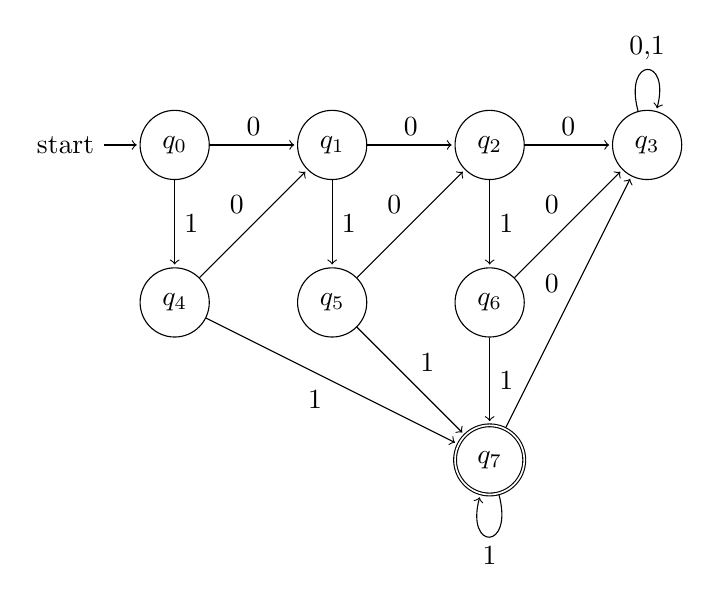
\begin{tikzpicture}[shorten >=1pt,node distance=2cm,on grid ,auto]
 \node[state ,initial] (q_0) {$q_0$};
 \node[state] (q_1) [right=of q_0] {$q_1$};
 \node[state] (q_2) [right=of q_1] {$q_2$};
 \node[state] (q_3) [right=of q_2] {$q_3$};
 \node[state] (q_4) [below=of q_0] {$q_4$};
 \node[state] (q_5) [below=of q_1] {$q_5$};
 \node[state] (q_6) [below=of q_2] {$q_6$};
 \node[state,accepting] (q_7) [below=of q_6] {$q_7$};
 \path[->]
  (q_0) edge node {0} (q_1) edge node {1} (q_4) 
  (q_1) edge node {0} (q_2) edge node {1} (q_5) 
  (q_2) edge node {0} (q_3) edge node {1} (q_6)
  (q_3) edge [loop above] node {0,1} ()
  (q_4) edge node {0} (q_1) edge node [swap] {1} (q_7)
  (q_5) edge node {0} (q_2) edge node {1} (q_7)
  (q_6) edge node {0} (q_3) edge node {1} (q_7)
  (q_7) edge node {0} (q_3) edge [loop below] node {1} ();
 \end{tikzpicture}
\subsection*{b.}

 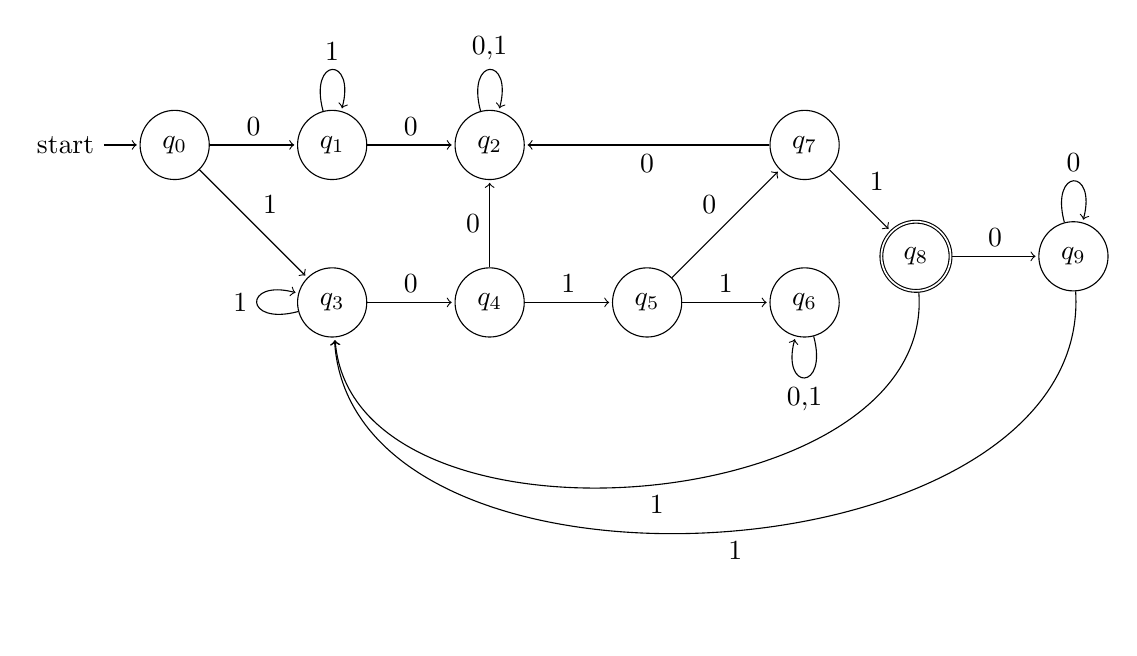
\begin{tikzpicture}[shorten >=1pt,node distance=2cm,on grid ,auto]
 \node[state ,initial] (q_0) {$q_0$};
 \node[state] (q_1) [right=of q_0] {$q_1$};
 \node[state] (q_2) [right=of q_1] {$q_2$};
 \node[state] (q_3) [below=of q_1] {$q_3$};
 \node[state] (q_4) [below=of q_2] {$q_4$};
 \node[state] (q_5) [right=of q_4] {$q_5$};
 \node[state] (q_6) [right=of q_5] {$q_6$};
 \node[state] (q_7) [above=of q_6] {$q_7$};
 \node[state,accepting] (q_8) [below right=of q_7] {$q_8$};
 \node[state] (q_9) [right=of q_8] {$q_9$};
 \path[->]
  (q_0) edge node {0} (q_1) edge node {1} (q_3) 
  (q_1) edge node {0} (q_2) edge [loop above] node {1} () 
  (q_2) edge [loop above] node {0,1} ()
  (q_3) edge [loop left] node {1} () edge node {0} (q_4)
  (q_4) edge node {0} (q_2) edge node {1} (q_5)
  (q_5) edge node {0} (q_7) edge node {1} (q_6)
  (q_6) edge [loop below] node {0,1} ()
  (q_7) edge node {0} (q_2) edge node {1} (q_8)
  (q_8) edge [bend left=90] node {1} (q_3) edge node {0} (q_9)
  (q_9) edge [loop above] node {0} () edge [bend left=90] node {1} (q_3);
 \end{tikzpicture}



\section*{Answer 5}

\subsection*{a.}
$$(q_0, abaa) \vdash _N (q_2, abaa) \vdash _N (q_4, baa) \vdash _N (q_4, aa) \vdash _N (q_1, a) \vdash _N (q_1, e)$$\\
$w_1\in L(N)$.
\subsection*{b.}
$$(q_0, babb) \vdash _N (q_1, abb) \vdash _N (q_1, bb)$$
$$(q_0, babb) \vdash _N (q_2, babb) \vdash _N (q_2, abb) \vdash _N (q_2, bb)\vdash _N (q_2, b)\vdash _N (q_2, e)$$
$$(q_0, babb) \vdash _N (q_2, babb) \vdash _N (q_2, abb) \vdash _N(q_4, bb) \vdash_N (q_4, b) \vdash_N (q_4,e)$$
$$(q_0, babb) \vdash _N (q_3, abb) \vdash _N (q_1, bb)$$
$$(q_0, babb) \vdash _N (q_3, abb) \vdash _N (q_4, abb) \vdash _N (q_1, bb)$$
$$(q_0, babb) \vdash _N (q_3, abb) \vdash _N (q_4, abb) \vdash _N (q_2, bb) \vdash _N (q_2,b) \vdash _N (q_2,e)$$
These are all possible configurations for $w_2$. Thus, $w_2\notin L(N)$.
\section*{Answer 6}
$E(q_0)=\{q_0,q_2\}$\\
$E(q_1)=\{q_1\}$\\
$E(q_2)=\{q_2\}$\\
$E(q_3)=\{q_3\}$\\
$E(q_4)=\{q_3,q_4\}$\\\\
$\delta(E(q_0), a)=E(q_0)=\{q_0,q_2\}$\\
$\delta(E(q_0), b)=E(q_0)\cup E(q_1)\cup E(q_3)=\{q_0,q_1, q_2, q_3\}$\\
$\delta(\{q_0,q_1, q_2, q_3\}, a)=E(q_0)\cup E(q_4)=\{q_0, q_2, q_3, q_4\}$\\
$\delta(\{q_0,q_1, q_2, q_3\}, b)=E(q_0)\cup E(q_1)\cup E(q_3)=\{q_0, q_1, q_2, q_3\}$\\
$\delta(\{q_0, q_2, q_3, q_4\}, a)=E(q_0)\cup E(q_4)=\{q_0, q_2, q_3, q_4\}$\\
$\delta(\{q_0, q_2, q_3, q_4\}, b)=E(q_0)\cup E(q_1)\cup E(q_3)=\{q_0, q_1, q_2, q_3\}$\\

 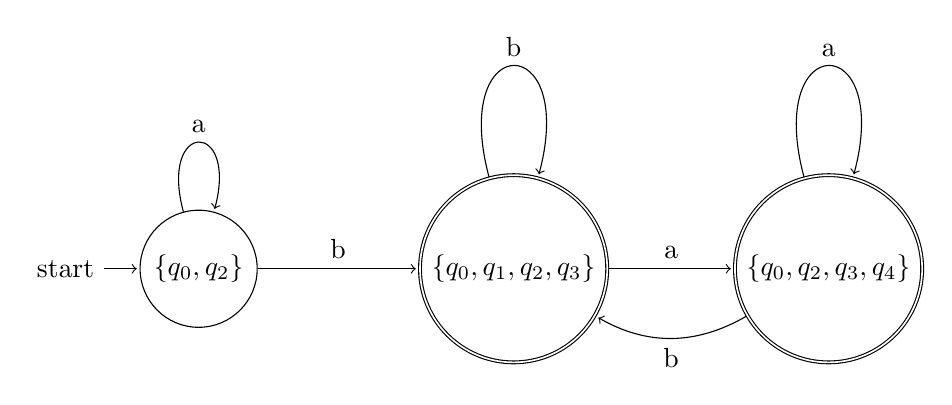
\begin{tikzpicture}[shorten >=1pt,node distance=4cm,on grid ,auto]
 \node[state ,initial] (X) {$\{q_0,q_2\}$};
 \node[state,accepting] (Y) [right=of X] {$\{q_0,q_1,q_2,q_3\}$};
 \node[state,accepting] (Z) [right=of Y] {$\{q_0,q_2,q_3,q_4\}$};
 \path[->]
 (X) edge [loop above] node {a} ()
 (X) edge node {b} (Y)
 (Y) edge [loop above] node {b} ()
 (Y) edge node {a} (Z)
 (Z) edge [loop above] node {a} ()
 (Z) edge [bend left] node {b} (Y);

 \end{tikzpicture}

\section*{Answer 7}
 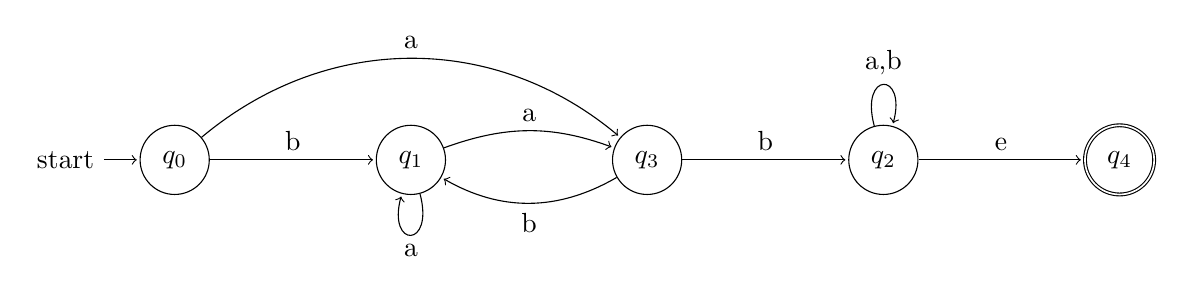
\begin{tikzpicture}[shorten >=1pt,node distance=3cm,on grid ,auto]
 
 \node[state ,initial] (q_0) {$q_0$};
 \node[state] (q_1) [right=of q_0] {$q_1$};
 \node[state] (q_3) [right=of q_1] {$q_3$};
 \node[state] (q_2) [right=of q_3] {$q_2$};
 \node[state,accepting] (q_4) [right=of q_2] {$q_4$};
 \path[->]
 (q_0) edge node {b} (q_1) edge [bend left=40] node {a} (q_3)
 (q_1) edge [loop below] node {a} () edge [bend left=20] node {a} (q_3)
 (q_2) edge [loop above] node {a,b} ()  edge node {e} (q_4)
 (q_3) edge [bend left] node {b} (q_1) edge node {b} (q_2)
 ;
 \end{tikzpicture}
 
\subsection*{a) Eliminate $q_1$}
$R(0,3,1)=ba^*a$\\
$R(3,3,1)=ba^*a$\\

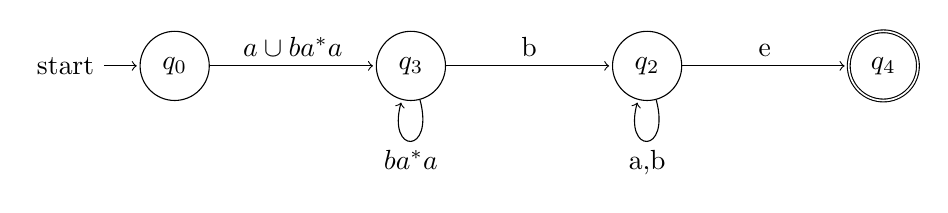
\begin{tikzpicture}[shorten >=1pt,node distance=3cm,on grid ,auto]
 
 \node[state ,initial] (q_0) {$q_0$};
 \node[state] (q_3) [right=of q_0] {$q_3$};
 \node[state] (q_2) [right=of q_3] {$q_2$};
 \node[state,accepting] (q_4) [right=of q_2] {$q_4$};
 \path[->]
 (q_0) edge node {$a\cup ba^*a$} (q_3)
 (q_2) edge [loop below] node {a,b} () edge node {e} (q_4)
 (q_3) edge [loop below] node {$ba^*a$} () edge node {b} (q_2)
 ;
 \end{tikzpicture}
 
\subsection*{b) Eliminate $q_2$}
$R(3,4,2)=b(a\cup b)^*e=b(a\cup b)^*$\\

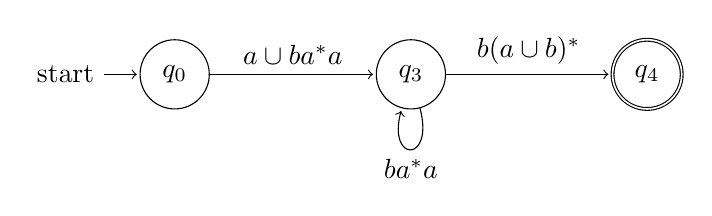
\begin{tikzpicture}[shorten >=1pt,node distance=3cm,on grid ,auto]
 
 \node[state ,initial] (q_0) {$q_0$};
 \node[state] (q_3) [right=of q_0] {$q_3$};
 \node[state,accepting] (q_4) [right=of q_3] {$q_4$};
 \path[->]
 (q_0) edge node {$a\cup ba^*a$} (q_3)
 (q_3) edge [loop below] node {$ba^*a$} () edge node {$b(a\cup b)^*$} (q_4)
 ;
 \end{tikzpicture}
 
\subsection*{c) Eliminate $q_3$}
$R(0,4,3)=(a\cup ba^*a)(ba^*a)^*(b(a\cup b)^*)$\\

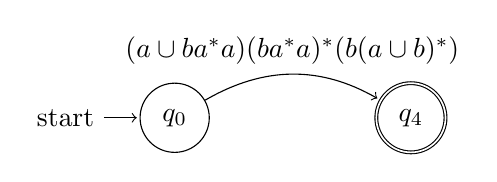
\begin{tikzpicture}[shorten >=1pt,node distance=3cm,on grid ,auto]
 
 \node[state ,initial] (q_0) {$q_0$};
 \node[state,accepting] (q_4) [right=of q_0] {$q_4$};
 \path[->]
 (q_0) edge [bend left] node {$(a\cup ba^*a)(ba^*a)^*(b(a\cup b)^*)$} (q_4)
 ;
 \end{tikzpicture}
 \\\\
 Regular expression is $(a\cup ba^*a)(ba^*a)^*(b(a\cup b)^*)$.
 
\section*{Answer 8}
Assume that $M_L=(K, \Sigma, \delta, q_0, F)$ and $M_H=(K', \Sigma, \delta ', s, F')$. I could not draw $M_L$ in a single picture as in our textbook on page 77 so I can just show the beginning part of it. \\

\begin{tikzpicture}[shorten >=1pt,node distance=3cm,on grid ,auto]
 
 \node[state ,initial] (q_0) {$q_0$};
 \node[state] (q_2) [below right=of q_0] {$q_2$};
 \node[state] (q_1) [above right=of q_0] {$q_1$};
 \path[->]
 (q_0) edge node {0} (q_1) edge node {1} (q_2)
 ;
 \end{tikzpicture}
 \\\\
 The starting state of $M_H$ must be $q_1$ and the accepting states are the ones who have outgoing transition with symbol 1 to any of final states of $M_L$. If $0w1 \in L$, then $(q_0,0w1)\vdash_{M_L}^*(f,e)$ for some $f\in F$ if and only if $(q_1,w1)\vdash_{M_L}^*(f,e)$ and $(s,0w)\vdash_{M_L}^*(f',1)$ for some $f'\in F'$. Hence, $M_L$ accepts $0w1$ if and only if $M_H$ accepts $w$. Thus, $L(M_H)=H$.
 

\section*{Answer 9}

\subsection*{a.}
Assume L is regular. There is an integer $p \geq 1$ such that any string $w\in L$ with $|w|\geq p$ can be written as $w=xyz$ such that $y\neq e,|xy|\leq p$ and $xy^kz\in L$ for each $k\geq 0$.\\
Let
$$x=1^t0^i$$
$$y=0^j$$
$$z=0^{p!-i-j}1^{2^{(p+1)!}}$$
for $0<j\leq p$. Then,
$$xy^kz=1^t0^{p!+(k-1)j}1^{2^{(p+1)!}}$$
If $p!+(k-1)j=(p+1)!$ then $n=m$. Let's see if the first equation holds for any $k$.
$$k-1=\frac{p!p}{j}$$
Since $j\leq p$, we can divide $p!$ by $j$ and there exists an integer k. This is a contradiction. Thus, L is not regular. 
\end{document}

​

